\documentclass[12pt]{article}
\usepackage{times} 			% use Times New Roman font

\usepackage[margin=1in]{geometry}   % sets 1 inch margins on all sides
\usepackage{hyperref}               % for URL formatting
\usepackage[pdftex]{graphicx}       % So includegraphics will work
\setlength{\parskip}{1em}           % skip 1em between paragraphs
\usepackage{indentfirst}            % indent the first line of each paragraph
\usepackage{datetime}
\usepackage[small, bf]{caption}
\usepackage{listings}               % for code listings
\usepackage{xcolor}                 % for styling code
\usepackage{multirow}
\usepackage{xurl} 
\usepackage{enumitem}
\usepackage[section]{placeins}
\usepackage{float}
\usepackage{hyperref}

%New colors defined below
\definecolor{backcolour}{RGB}{246, 246, 246}   % 0xF6, 0xF6, 0xF6
\definecolor{codegreen}{RGB}{16, 124, 2}       % 0x10, 0x7C, 0x02
\definecolor{codepurple}{RGB}{170, 0, 217}     % 0xAA, 0x00, 0xD9
\definecolor{codered}{RGB}{154, 0, 18}         % 0x9A, 0x00, 0x12

%Code listing style named "gcolabstyle" - matches Google Colab
\lstdefinestyle{gcolabstyle}{
  basicstyle=\ttfamily\small,
  backgroundcolor=\color{backcolour},   
  commentstyle=\itshape\color{codegreen},
  keywordstyle=\color{codepurple},
  stringstyle=\color{codered},
  numberstyle=\ttfamily\footnotesize\color{darkgray}, 
  breakatwhitespace=false,         
  breaklines=true,                 
  captionpos=b,                    
  keepspaces=true,                 
  numbers=left,                    
  numbersep=5pt,                  
  showspaces=false,                
  showstringspaces=false,
  showtabs=false,                  
  tabsize=2
}

\lstset{style=gcolabstyle}      %set gcolabstyle code listing

\makeatletter
\g@addto@macro{\UrlBreaks}{\UrlOrds}
\makeatother

% for fancy page headings
\usepackage{fancyhdr}
\setlength{\headheight}{13.6pt} % to remove fancyhdr warning
\pagestyle{fancy}
\fancyhf{}
\rhead{\small \thepage}
\lhead{\small HW8, Lewis}  
\chead{\small CS 432, Fall 2020} 

%-------------------------------------------------------------------------
\begin{document}

\begin{centering}
{\large\textbf{HW8 - Clustering}}

Brenden Lewis\\                     
Due: 12/6/2020 11:59PM\\                      
\end{centering}

%-------------------------------------------------------------------------
\section*{Q1}
Listing 1 below shows the Python code used to collect Twitter data needed for the assignment. I utilized the Tweepy library to collect tweets across my chosen accounts. When choosing accounts to collect data from, I initially looked at a list of the Top 100 most followed accounts of all time on Twitter and started from there. The lists I looked at had total tweet counts across the accounts and they all happened to be verified, so I chose all the accounts that fit the criteria; after filtering the Top 100 list, I had about 40 accounts collected. 

\par I was not able to figure out how to automate finding accounts through Tweepy, so I opted to get the remaining accounts \emph{semi}-manually. What I mean by that is I had to identify accounts that I knew were extremely popular, checking if they were verified, and double-checking their follower counts. These accounts included musicians, celebrities, businesses, restaurants, sports players and networks, streaming services, and random comedy accounts. I did this in batches, as I had to take screen names of the accounts and run them through tweepy to check their tweet counts; this was handled in the \emph{collectAccounts()} method. Each account I scanned that were over the 5000+ tweets threshold was added to the collection.  

\lstinputlisting[language=Python, caption= Python code used to collecting tweets for Q1, label=lst:import]{collectTweets.py}

Listing 2 below shows the final list of accounts used for tweet processing. This collection was processed in the \emph{retrieveTweets()} method to collect the 200 most recent tweets from each account. When pulling tweets from each account's timeline, I found I had to add the parameter \emph{tweet\textunderscore mode = "extended"} to the \emph{api.user.timeline()} call to pull the full tweet, otherwise only a snippet of the tweet would be pulled.

\begin{lstlisting}[language=Python, caption={100 Accounts used}, label=lst:copy]
BarackObama
justinbieber
katyperry
rihanna
realDonaldTrump
ladygaga
ArianaGrande
TheEllenShow
YouTube
KimKardashian
selenagomez
CNN
ddlovato
shakira
jimmyfallon
KingJames
nytimes
MileyCyrus
JLo
Oprah
NASA
BeingSalmanKhan
elonmusk
KevinHart4real
wizkhalifa
KylieJenner
espn
KendallJenner
aliciakeys
HillaryClinton
pitbull
NatGeo
coldplay
Google
MariahCarey
NICKIMINAJ
davidguetta
ricky_martin
JERICHO
SavinTheBees
NBA
WHO
Ninja
PostMalone
TheDailyShow
FoxNews
matthewmercer
hulu
netflix
adamlevine
NFL
MLB
TheRock
WNBA
Sony
Microsoft
Windows
NHL
NintendoAmerica
NintendoUK
PaulMcCartney
FIFAcom
EA
Blizzard_Ent
RealRonHoward
BigMikeJ73
michaelb4jordan
BET
BETMusic
bethesda
WuTangClan
AOC
NathanFillion
ToddHaberkorn
TroyBakerVA
WayneBrady
Crunchyroll
Wendys
dominos
tacobell
McDonalds
BurgerKing
PapaJohns
littlecaesars
pizzahut
MrPeanut
RoosterTeeth
Monstercat
PegboardNerds
StephenAtHome
KenJennings
TheTweetOfGod
TheOnion
Bungie
Treyarch
Respawn
Charmin
marshmellomusic
MerriamWebster
BaskinRobbins
\end{lstlisting}

Each tweet was stored as a dictionary containing the tweet ID and the full body of text. This dictionary was then appended to a list for each user, which then another dictionary was created for each user containing their screen name and list of tweets. After all the tweets were pulled for a single account, the screen name and tweets were passed to \emph{writeTweetsToFile()} to automatically write a text file containing each tweet for each account. Each of these final user collections were then combined to a single list of dictionaries to exported to JSON for processing later.

\par Listing 3 below shows the first few tweets pulled from Barack Obama's account \emph{@BarackObama} and their IDs. 

\begin{lstlisting}[language=Python, caption={Sample of tweets pulled from Barack Obama's account}, label=lst:copy]
1336679633769680898
In A Promised Land, I talk about the decisions I had to make during the first few years of my presidency. Here are some thoughts on how I approach tough questions: https://t.co/GFumGnNPln

1336370071917240321
With COVID-19 cases reaching an all-time high this week, we've got to continue to do our part to protect one another. This pandemic is far from over and your actions can help save lives. https://t.co/XJ4dbsCihB

1335954913344565258
To all of you in Georgia, today is the last day to register to vote in the upcoming runoff election. Take a few minutes right now to register to vote, and then make sure everybody you know is registered, too. https://t.co/2Ob571igh3 https://t.co/SslnFSWMfi
\end{lstlisting}

\section*{Q2}
Listing 4 below is code used for processing the collected tweets, their text, collecting the final data needed to form the account-term matrix.

\par The first step was to read in the accounts and JSON file containing the tweets. Once read-in, the method \emph{matchTweets()} was used to organize the tweets by creating a nested list \emph{tweets\textunderscore per\textunderscore account} containing each list of 200 tweets with the same index as the account the came from in the \emph{accounts} list (so tweets\textunderscore per\textunderscore account[0] contains the list of tweets from the account at accounts[0])

\par The next step was to simultaneously gather the words from each tweet, clean them, and store them in another nested list \emph{words\textunderscore per\textunderscore account} to store the tweet words with their respective account index. Cleaning the tweets means removing any links, punctuation, account mentions, emojis, and any non-alpha character. The \emph{cleanText()} method was called for each tweet, which lower cased each tweet, used regular expressions to remove the unneeded content, and ran an additional check to remove words less than 3 characters and more than 15 characters. The clean collection of words is then appended to \emph{words\textunderscore per\textunderscore account} before moving onto the next user's tweets.

\par Once the the tweets were cleaned and there was collection of words for each account, I needed to fake removing stopwords with the \emph{fakeStopwordsTFIDF()} method. But before I could call that method, I needed a dictionary containing each word and how many accounts had tweets containing that word for calculation; \emph{getAPCount()} was used to build this dictionary. The easiest way I found was to use list comprehension to build a list of all words per account excluding duplicate entries and using \emph{dictionary.get()} to either add the word with a default count to the dictionary or increment the count of the word if it already exists in the dictionary. This final dictionary was then sorted in descending order by the number of accounts each word appeared in.

\par The \emph{apcount} was then passed into \emph{fakeStopwordsTFIDF()}. This method simulated TFIDF calculations for each word to remove stopwords from the overall list of words. This returned a new list containing words that appeared in more than 10\% and fewer than 50\% of the accounts. With this final list of words, it was time to count the frequency of each word across all tweets using \emph{countFinalWords()}. Using similar logic to getting \emph{apcount}, each final word was compared across all tweets per account and appended to a new dictionary using \emph{dictionary.get()} to increment the frequency for duplicate occurrences. 

\textbf{Of note, I'm aware my method for iterating through each word is extremely inefficient, but by this point it was much faster for me to process it the way I did than to go back and properly reorganize my data structures.}

\par Finally, this dictionary of words was sorted by frequency counts in descending order. From this sorted dictionary, the first 1000 terms (top 1000 most common words) were stored in a final dictionary. With this list, the \emph{createMatrix()} method was called to create a two-dimensional list \emph{matrix} containing rows with the final words and their frequency across each account. For each account, a \emph{row} dictionary was created containing each of the 1000 terms and a default value of 0. Cross referencing each term within \emph{row} with all words across all tweets from the current account, the term's frequency count was incremented each time a match occurred. This row was then appended to \emph{matrix}.

\lstinputlisting[language=Python, caption=Python code used for word processing in Q2, label=lst:import]{q2.py}

\par The final 2D list of data \emph{matrix} was then exported to JSON for use in another file to build the physical matrix. Listing 5 below shows an extremely small beginning snippet of the JSON file, highlighting the first 25 most common terms across all tweets and their frequency in tweets posted by \emph{@BarackObama}.  

\begin{lstlisting}[language=Python, caption={First 25 terms for @BarackObama in MatrixData.json}, label=lst:copy]
[
  {
    "sorry": 0,
    "election": 44,
    "covid19": 3,
    "app": 0,
    "christmas": 0,
    "song": 0,
    "details": 0,
    "birthday": 0,
    "phone": 1,
    "store": 0,
    "trump": 0,
    "address": 1,
    "news": 1,
    "location": 0,
    "nba": 4,
    "name": 1,
    "collection": 1,
    "games": 0,
    "email": 0,
    "december": 1,
    "via": 0,
    "health": 13,
    "care": 17,
    "album": 0,
    "order": 0,
\end{lstlisting}

Listing 6 below shows the code used to draw and export the final account-term matrix. The matrix data from \emph{q2.py} and the list of accounts was read in and stored within the file. To assist with creating the matrix, the matrix data in particular was appended to a new list with each "row" of data being attached to the account name it belonged to (which was easy considering the row of data and it's associated account shared the same index value in their respective lists). With this list structure, the list could easily be passed into \emph{pd.DataFrame().T} to create a transposed data frame to represent the account-term matrix.

While the final matrix is extremely large and can't be fully represented in this report, printing the table in my IDE shows an extremely condensed, more easily readable version of the table, shown in Listing 7. 

\lstinputlisting[language=Python, caption=Python code used to draw the account-term matrix after processing, label=lst:import]{drawMatrix.py}

\begin{lstlisting}[language=Python, caption={Condensed account-term matrix captured in output}, label=lst:copy]
                 sorry  election  covid19   ...  present  finish  blast
BarackObama          0        44        3   ...        0       0      0
justinbieber         0         0        0   ...        0       0      0
katyperry            2         4        0   ...        1       0      0
rihanna              0         0        1   ...        0       0      0
realDonaldTrump      0         5        0   ...        0       0      0
...                ...       ...      ...   ...      ...     ...    ...
Respawn              0         0        0   ...        1       1      0
Charmin              4         0        0   ...        0       0      1
marshmellomusic      0         0        0   ...        2       1      0
MerriamWebster       0         1        0   ...        0       0      0
BaskinRobbins       67         0        0   ...        0       0      1

[100 rows x 1000 columns]
\end{lstlisting}

\section*{Q3}
Listing 8 below shows all the code involved in all forms of clustering and drawing graphs; this code is used for answering the remaining questions. The large majority of this code pulled from the example code with some minor changes for reading in data and output.

\par My resulting account-term matrix was read-in through \emph{readFile()}. Within this function, the matrix was stripped apart to get the screen names, the 1000 terms, and a 2-dimensional array of data containing the frequency counts for each word in each account. These three lists were returned and stored to be used for clustering algorithms. 

\lstinputlisting[language=Python, caption=Python code to handle all clustering and dendrograms, label=lst:import]{drawClusters.py}

\par The method \emph{hcluster()} takes the data array and creates the hierarchical clusters of the accounts. This list of clusters is passed to \emph{printclust()} to print an ASCII dendrogram of the clusters. Figure 1 below shows a small snapshot of the ASCII dendrogram, showcasing it's hierarchical structure. \emph{drawdendrogram()} was then called to create a JPEG image of a new set of clusters created by calling \emph{hcluster()} again after rotating the data array with \emph{rotatematrix()} (rotating the array was only needed to print a vertical dendrogram like the ASCII dendrogram). The resulting dendrogram is shown in Figure 2; the image itself was both massive and extremely long, so I took cropped snapshot of the very top of the dendrogram to showcase. 

\begin{figure}[H]
            \centering
            \includegraphics[scale=1.0,trim = 0 0 0 0, clip]{ascii_snip.png}
            \caption{Snippet of ASCII dendrogram}
            \label{fig:my_label}
        \end{figure}

\begin{figure}[H]
            \centering
            \includegraphics[scale=0.60,trim = 0 0 100 0, clip]{clusters_snip.jpg}
            \caption{Snippet of dendrogram}
            \label{fig:my_label}
        \end{figure}

\section*{Q4}
Clustering the accounts using k-means was done through the \emph{kcluster()} method which takes the data array and a \emph{k} value as parameters. I called the method three times for k=5, k=10, and k=20, and wrote the resulting account clusters to their own files.

Listing 9 below shows the number of iterations taken for each k-value. At k=5, five iterations were needed to cluster the accounts. At k=10, thirteen iterations were needed to cluster the accounts. At k=20, only four iterations were needed to cluster the accounts.

\begin{lstlisting}[language=Python, caption={Iterations for each k-value}, label=lst:copy]
For k=5
Iteration 0
Iteration 1
Iteration 2
Iteration 3
Iteration 4
Iteration 5

For k=10
Iteration 0
Iteration 1
Iteration 2
Iteration 3
Iteration 4
Iteration 5
Iteration 6
Iteration 7
Iteration 8
Iteration 9
Iteration 10
Iteration 11
Iteration 12
Iteration 13

For k=20
Iteration 0
Iteration 1
Iteration 2
Iteration 3
Iteration 4
\end{lstlisting}

Listing 10 shows the different account clusters at k=5: 
\begin{itemize}
    \item The first cluster is primarily fast food accounts, but also features a sports network and voice actor account. 
    \item The second cluster is not too coherent, as it features a mix of political figures, celebrities, musicians, video game companies, and miscellaneous businesses. 
    \item The third cluster is very similar to the second, featuring a mix of celebrities, musicians, streaming services, influencers, and sports networks.
    \item The fourth cluster can't really be characterized as it only contains 5 members who are all different from one another.
    \item The fifth cluster predominantly features news websites, the remaining political figures, and parody accounts.
\end{itemize}

\begin{lstlisting}[language=Python, caption={Clustering at k=5}, label=lst:copy]
Iterations at k=(5):  5

matthewmercer
NFL
Wendys
dominos
McDonalds
BurgerKing
PapaJohns
pizzahut
BaskinRobbins

BarackObama
ladygaga
selenagomez
ddlovato
shakira
Oprah
NASA
elonmusk
HillaryClinton
pitbull
NatGeo
ricky_martin
WHO
Microsoft
NintendoAmerica
EA
Blizzard_Ent
bethesda
WuTangClan
littlecaesars
Bungie
Treyarch
Respawn
Charmin

justinbieber
katyperry
rihanna
ArianaGrande
TheEllenShow
YouTube
KimKardashian
KingJames
MileyCyrus
JLo
BeingSalmanKhan
KevinHart4real
wizkhalifa
KylieJenner
KendallJenner
aliciakeys
coldplay
MariahCarey
NICKIMINAJ
davidguetta
JERICHO
SavinTheBees
Ninja
PostMalone
hulu
netflix
adamlevine
MLB
TheRock
WNBA
Sony
NintendoUK
FIFAcom
michaelb4jordan
BET
BETMusic
NathanFillion
TroyBakerVA
WayneBrady
tacobell
MrPeanut
RoosterTeeth
Monstercat
PegboardNerds
marshmellomusic
MerriamWebster

espn
Google
NBA
Windows
PaulMcCartney

realDonaldTrump
CNN
jimmyfallon
nytimes
TheDailyShow
FoxNews
NHL
RealRonHoward
BigMikeJ73
AOC
ToddHaberkorn
Crunchyroll
StephenAtHome
KenJennings
TheTweetOfGod
TheOnion
\end{lstlisting}

Listing 11 shows the different account clusters at k=10: 
\begin{itemize}
    \item The first cluster seems to be related to current politics.
    \item The second cluster has a good mix of celebrities, musicians, and game companies; nothing to specific. 
    \item The third cluster is similar to the last, being a list of celebrities, musicians, and game companies. 
    \item The fourth cluster is primarily actors, musicians, and game companies, however, these actors and musicians often interact together such as Kevin Hart and Dwayne Johnson, and Justin Bieber and Selena.
    \item The NHL is it's own cluster for some reason, when ideally it would be grouped with the other sports networks.
    \item The sixth cluster is probably the most focused in this set. The cluster is largely comprised of accounts related to music, streaming, and games. There are some unrelated famous figures mixed in such as LeBron James, Michael B. Jordan (the actor), and Wayne Brady. 
    \item The seventh cluster is mostly fast food restaurants, but the other half of the accounts are unrelated to either restaurants nor each other.
    \item The last three clusters aren't at all coherent and are quite small. So it's difficult to determine how they could be clustered together.
\end{itemize}

\begin{lstlisting}[language=Python, caption={Clustering at k=10}, label=lst:copy]
Iterations at k=(10):  13

realDonaldTrump
CNN
nytimes
NatGeo
TheDailyShow
FoxNews
AOC
ToddHaberkorn
TheTweetOfGod
TheOnion

BarackObama
ladygaga
TheEllenShow
YouTube
ddlovato
Oprah
NASA
elonmusk
HillaryClinton
bethesda
NathanFillion
tacobell
StephenAtHome
Treyarch
marshmellomusic

KimKardashian
shakira
KylieJenner
KendallJenner
pitbull
ricky_martin
WHO
Microsoft
NHL
PaulMcCartney
EA
Blizzard_Ent
WuTangClan
littlecaesars
MrPeanut
KenJennings
Bungie
Respawn

justinbieber
selenagomez
BeingSalmanKhan
KevinHart4real
TheRock
NintendoAmerica
NintendoUK
RoosterTeeth

NFL

katyperry
rihanna
ArianaGrande
KingJames
MileyCyrus
JLo
wizkhalifa
aliciakeys
coldplay
MariahCarey
NICKIMINAJ
davidguetta
JERICHO
SavinTheBees
Ninja
PostMalone
hulu
netflix
adamlevine
Sony
michaelb4jordan
BET
BETMusic
TroyBakerVA
WayneBrady
Monstercat
PegboardNerds

matthewmercer
Windows
RealRonHoward
Wendys
dominos
McDonalds
PapaJohns
Charmin
MerriamWebster
BaskinRobbins

WNBA
BigMikeJ73
BurgerKing
pizzahut

jimmyfallon
espn
NBA
Crunchyroll

Google
MLB
FIFAcom
\end{lstlisting}

Listing 12 shows the different account clusters at k=20. Most the of the clusters for k= 20 are quite small, with some only containing a single account. I do want to highlight a few clusters I believe to be quite accurate: 
\begin{itemize}
    \item The very first cluster with @KevinHart4Real and @TheRock makes sense, as these two are both good friends and have appeared together in many popular movies.
    \item The seventh cluster includes all the athletes alongside the @espn sports network. The others in that cluster share very similar Twitter personalities.  
    \item The thirteenth cluster houses all accounts with political affiliation and news outlets (outside of Little Caesars Pizza, unsure about that one). These accounts may have tweeted heavily in regards to the most recent election. 
    \item The sixteenth cluster is small, but groups @NASA and @elonmusk together, which makes sense given their involvement in space programs.
    \item The final cluster is the largest, but also almost entirely made up of popular musicians and music streaming platforms; the only oddballs are @WHO (World Health Organization) and @NatGeo 
    
\end{itemize}

\begin{lstlisting}[language=Python, caption={Clustering at k=20}, label=lst:copy]
Iterations at k=(20):  4


KevinHart4real
TheRock

Google
NHL
NintendoUK
dominos

NathanFillion
TheTweetOfGod
Treyarch

NFL

Microsoft

MariahCarey
JERICHO
Ninja
bethesda

rihanna
KingJames
espn
NICKIMINAJ
SavinTheBees
BigMikeJ73
michaelb4jordan

wizkhalifa
PapaJohns
MrPeanut
StephenAtHome

ArianaGrande
shakira
BeingSalmanKhan
matthewmercer
netflix
WNBA
Sony
WuTangClan
BaskinRobbins

TheEllenShow
KendallJenner
MLB
FIFAcom
EA
BETMusic
Bungie
Charmin

pitbull
hulu
NintendoAmerica
PaulMcCartney
RealRonHoward
Respawn

NBA

BarackObama
realDonaldTrump
ladygaga
CNN
nytimes
Oprah
HillaryClinton
TheDailyShow
FoxNews
AOC
littlecaesars
TheOnion

jimmyfallon
BET
ToddHaberkorn
Crunchyroll
tacobell

KimKardashian
KylieJenner
Wendys
McDonalds
BurgerKing
pizzahut
RoosterTeeth

NASA
elonmusk
MerriamWebster

Windows
Blizzard_Ent
TroyBakerVA
WayneBrady
PegboardNerds
KenJennings

justinbieber
katyperry
YouTube
selenagomez
ddlovato
MileyCyrus
JLo
aliciakeys
NatGeo
coldplay
davidguetta
ricky_martin
WHO
PostMalone
adamlevine
Monstercat
marshmellomusic
\end{lstlisting}

Comparing the different k-values and their results on the data, it appears to me that k = 20 is the most accurate value for clustering my data. While each value shared a number of inaccuracies in it's clustering, the clusters at k = 20 seem to make the most amount of sense. This comes as a surprise, as I was initially expecting k = 10 to provide the most accurate clusters.

\section*{Q5}

MDS was handled through both the \emph{scaledown()} and \emph{draw2d()} methods. \emph{scaledown()} took in the 2D array of data as an arguments and returned the coordinates of each account. These coordinates allowed the data to be clustered and plotted in a 3-dimensional format. Listing 13 shows a list of the total percent differences per iteration. Counting the output, a total of 92 iterations was needed to move each point the the best possible positions. 

\par This graph was plotted by passing the coordinates into \emph{draw2d()} alongside the list of accounts; this method used the imaging library \emph{Pillow} to plot and export the image. The final MDS image is shown below in Figure 3. Unfortunately, due to it's extreme size, it had to be scaled down to capture the full, 3-dimensional effect. 

\begin{figure}[H]
            \centering
            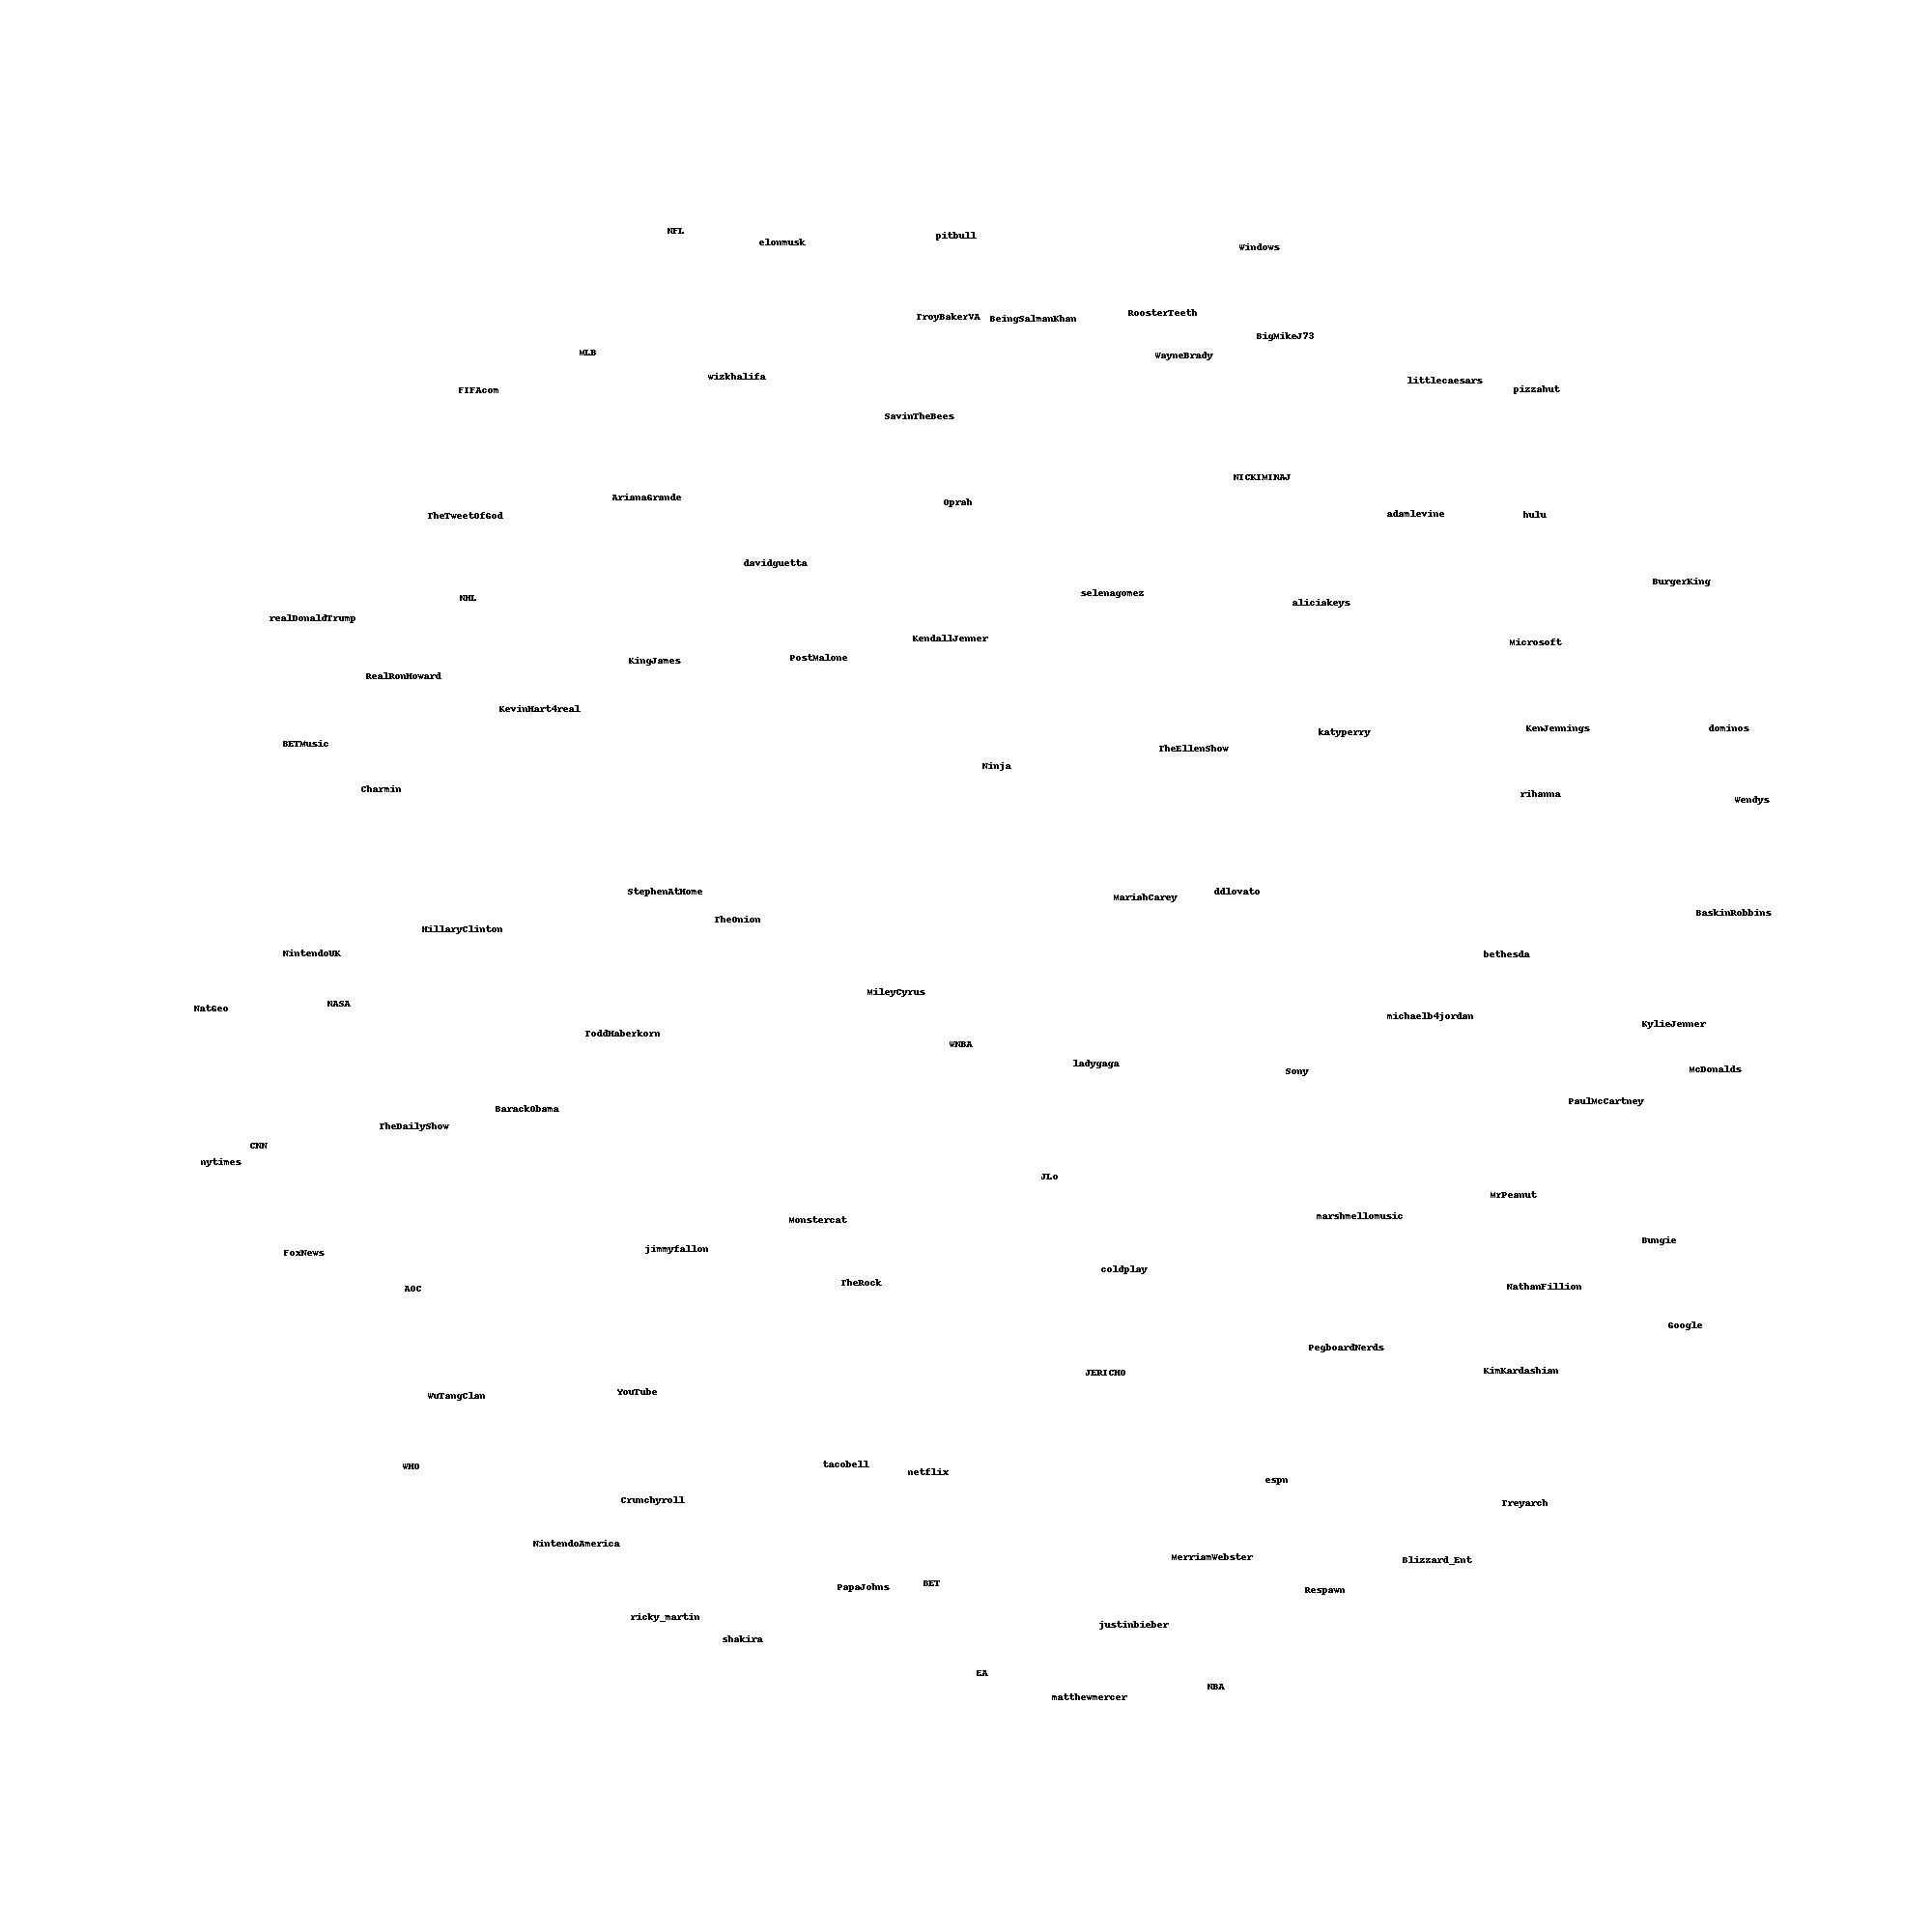
\includegraphics[scale=0.27,trim = 100 90 100 200, clip]{mds2d.jpg}
            \caption{MDS}
            \label{fig:my_label}
        \end{figure}
        
\begin{lstlisting}[language=Python, caption={Output from scaledown()}, label=lst:copy]
4292.093979274119
3468.6963378241735
3443.1605133694075
3433.8771891736046
3428.3435921231517
3424.1729984429485
3421.120766401213
3418.7469839225996
3416.4118497193167
3414.4440844275505
3412.440863751611
3410.6465210733254
3409.0135600255144
3407.828801597129
3406.614686573917
3405.348619533868
3403.879972210023
3402.4599352017785
3400.6049413304436
3398.4835025635516
3396.4503913590497
3394.498279149446
3392.6385673344253
3390.574933345304
3388.2408982400316
3385.945677397648
3383.644519964651
3381.3471770664746
3379.071768466391
3376.9061201468085
3374.86572041902
3372.7470693075834
3370.679695018536
3368.8020144909347
3367.078404372282
3365.4284726916517
3363.5180227427154
3361.5044352044524
3359.567836902659
3357.6994851742597
3356.075201494575
3354.6152534564762
3353.3437071308554
3352.335510480809
3351.321018381074
3350.1888786790323
3348.985883309517
3347.780406455964
3346.5534605142593
3345.199031162315
3343.751169397896
3342.243964528533
3340.5999192427143
3339.0387078681683
3337.450064806221
3335.923911769075
3334.5058497032032
3333.1150908016352
3331.899056124837
3330.6460139440615
3329.390198500818
3328.2085720215514
3326.942245522004
3325.6903331491635
3324.731009673131
3323.9414807388216
3323.252399237465
3322.621871481046
3321.966053962298
3321.3863407367453
3320.7252626481722
3320.1258695526835
3319.5913971475425
3319.042673119391
3318.3179305943013
3317.530619079285
3316.6666483553036
3315.6227629071536
3314.6336580402417
3313.929465632325
3313.255518125941
3312.461244955732
3311.738311092058
3310.991010500956
3310.235490785789
3309.330568837568
3308.2826330791786
3307.2518796395166
3306.6054579567126
3305.799861116069
3305.253415207178
3305.255269419066
\end{lstlisting}

\section*{Q7 (Extra)}
Figure 4 below shows an alternate version of the dendrogram shown in Figure 2 using the same data. This version of the dendrogram was generated using the \emph{plotly.figure\textunderscore facory} library and the \emph{create\textunderscore dendrogram()} method.
In order to get a clear view of the words, the image height had to be scaled up considerably to the point where it would be impossible to pass into this report. I trimmed and scaled it to best capture the overall shape from a portion of the final dendrogram.
\begin{figure}[H]
            \centering
            
\includegraphics[scale=0.15,trim = 9 8500 0 0, clip]{clusters_plotly.png}
            \caption{Snippet of dendrogram plotted using Plotly}
            \label{fig:my_label}
        \end{figure}

\section*{Q8 (Extra)}
Using the same coordinate gathering method for each account from Q5, I created a scatter plot mimicking the generated MDS figure. This was done using the \emph{matplotlib.pyplot} library within the \emph{draw2dAgain()} method. All the x and y-axis values were captured and passed to \emph{plt.scatter()}, with \emph{plt.text()} to attach the account labels to each point. Due to running \emph{scaledown()} again for this graph, the points are not in the same position as the original MDS figure.

\begin{figure}[H]
            \centering
            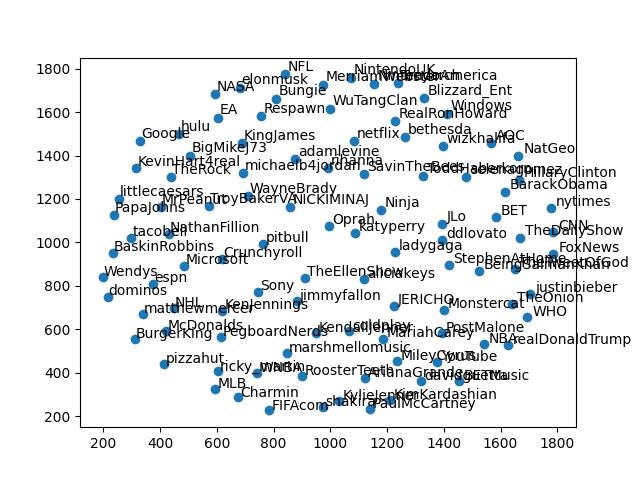
\includegraphics[scale=1.0,trim = 0 0 0 0, clip]{mds_pyplot.png}
            \caption{MDS plotted using PyPlot}
            \label{fig:my_label}
        \end{figure}

\end{document}
